\documentclass[11pt]{article}

\title{Lambda Lifting Transformation}
\usepackage[utf8]{inputenc}
\usepackage{tikz}
\usepackage{tikz-3dplot}
\usepackage{tikz-cd}
\usepackage{xcolor}
\usepackage{proof}
\usepackage {alltt}

\usepackage{graphicx} % Allows including images
\usepackage{booktabs} % Allows the use of \toprule, \midrule and \bottomrule in tables
\usepackage{listings}
\usepackage[export]{adjustbox}
\usepackage{verbatim}
\tikzset
  {cross/.style={cross out, draw=black, minimum size=2*(#1-\pgflinewidth), inner sep=0pt, outer sep=0pt},cross/.default={1pt}}


\usepackage{amsmath }
\usepackage{framed}
\usepackage{proof}
\usepackage{enumerate,xspace,stmaryrd}
\usepackage{amsmath,amssymb,latexsym}
\usepackage{textcomp,xspace}
\usepackage[top=2cm, bottom=2.5cm, right=2.5cm, left=2.5cm]{geometry}\usepackage{latexsym}  %For plain TeX symbols, such as \Box used in \qed
\usepackage{euscript}  %%Euler Script font
\usepackage {mdframed}
\usepackage{ifpdf}
\usepackage {alltt}
\renewcommand{\ttdefault}{txtt}
\ifpdf
  \usepackage{epstopdf}
\fi 
\usepackage{etoolbox}
\BeforeBeginEnvironment{tabular}{\begin{center}\small}
\AfterEndEnvironment{tabular}{\end{center}}

\tikzstyle{stage} = [rectangle,minimum width=2.8cm,rounded corners,
                     minimum height=1.8cm,text centered, draw=black]
\tikzstyle{arrow} = [very thick,->,>=stealth]

\begin{document}

\maketitle
\section {Lambda Lifting} 
Once pattern-matching compilation is completed, the next step in the interpretation of MPL programs is lambda lifting. MPL allows the programmers to define local functions. However, Core MPL doesn't allow for local function definitions. Thus all the local MPL functions must be put in the global scope. Lambda lifting is the transformation that puts the local functions in the global scope. The {\sf defn} and {\sf where} are the two MPL constructs that allow for local function definitions. 
~~\\~~\\ 
In this chapter, the difference between the {\sf defn} and {\sf where} constructs, and the strategy for lambda lifting of each contruct is discussed. An algorithm for lambda lifting was given Thomas Johnsson. The algorithm described in the chapter is an adaptation of Johnsson's algorithm customised for MPL.
\begin{figure}[!h]
\begin {center}
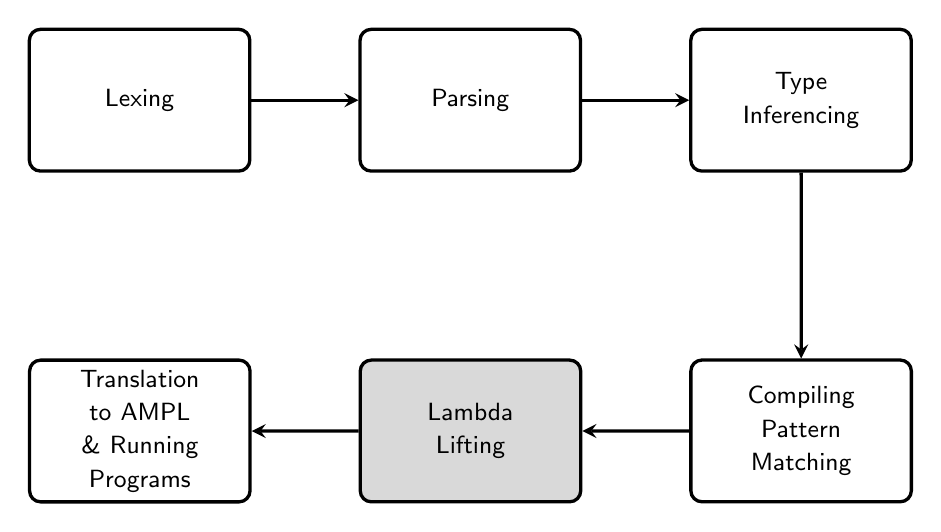
\begin{tikzpicture}[scale = 1.5,every node/.style={very thick},node distance=2cm]
 \node (LE) [stage] {{\sf \small Lexing}};
 \node (PA) [stage,right of=LE,xshift=2.2cm] {{\sf \small Parsing}};
 \node (TC) [stage,right of=PA,xshift=2.2cm,text width = 1.8cm] {{\sf \small Type Inferencing}};
 \node (CP) [stage,below of=TC,yshift=-2.2cm,text width = 1.8cm] 
            {{\sf \small Compiling Pattern Matching}};
 \node (LL) [stage,left of=CP,xshift=-2.2cm,text width = 1.8cm,fill=gray!30] 
            {{\sf \small Lambda Lifting}};
 \node (AM) [stage,left of=LL,xshift=-2.2cm,text width = 1.8cm] 
            {{\sf \small Translation to AMPL \& Running Programs}};
 \draw [arrow] (LE) -- (PA);
 \draw [arrow] (PA) -- (TC);
 \draw [arrow] (TC) -- (CP);
 \draw [arrow] (CP) -- (LL);
 \draw [arrow] (LL) -- (AM);
\end{tikzpicture}
\caption{Interpretation Stages of MPL} \label{fig:CSAM}
\end{center}
\end{figure}



\section {Local Function Definitions with defn and where Constructs}
Although both {\sf defn} and {\sf where} can be used to define local functions, there is a significant difference these constructs: the {\sf defn} construct doesn't allow local variables while the main of the {\sf where} construct is to allow non local variables. This has been described in Section \ref {lam:defnOverview} and Section \ref {lam:whereOverview} with examples.

\subsection {defn Construct}\label{lam:defnOverview}
The {\sf defn} construct is used to modularize programs in MPL. Table \ref {lam:defnExample} shows an example of a pattern matching compiled MPL program that uses the {\sf defn} construct. The program takes two lists and returns backs a list where each element of the final list is the sum of the corresponding elements of the original list. In case of lists of unequal length, the sum of the corresponding elements is calculated till the elements in the smaller list is exhausted and the remaninder of the elements in the longer list are ignored. 
~~\\~~\\
As can be seen in Table \ref {lam:defnExample}, {\sf defn} consists of two components:
\begin{itemize}
  \item {\bf Main body of defn}: MPL definitions between the keywords {\bf defn} and {\bf where} form the main body of {\sf defn}. These definitions can be (co)data, (co)protocol, process, or function definitions. These definitions are visible to the entire MPL program.

  \item {\bf where clause of defn}: There may be some definitions that are required only for the definitions in the main body of the {\sf defn} construct. These definitions are written in the {\bf where} clause of the {\sf defn} construct. Scope of a definition in the {\bf where} clause of {\sf defn} is:
  \begin{itemize}
    \item other definitions in the where clause, and
    \item the definitions in the main body of the {\sf defn} construct.
  \end{itemize}
\end{itemize}
For example, in Table \ref {lam:defnExample}, the {\bf List} data type is in the scope of functions {\bf helperfun}, and {\bf zipSum} and not in scope of {\bf mainFun}. Similarly, function {\bf helperFun} is in the scope of function {\bf zipSum} and not in the scope of {\bf mainFun}. Function {\bf zipSum} is in scope of function {\bf mainFun}. Thus MPL uses {\sf defn} construct to implement data hiding and to control the visibility of definitions.
~~\\ ~~\\
In Section \ref {lam:algDefn}, the lambda lifting algorithm for the {\sf defn} construct is discussed.

\begin{table}[!h]
\begin{center}
\begin{tabular}{|c|} \hline
\begin{minipage}{5in}
\begin{alltt}


  fun mainFun = 
      x,y -> zipSum(x,y)
  
  defn
    fun zipSum =
      x,y -> helperFun (x,y)
  where 
    data List(A) -> C = Nil  ::     -> C
                        Cons :: A,C -> C 

    fun helperFun 
      l1,l2 ->
        case l1 of 
          Nil -> Nil
          Cons(x,xs) -> case l2 of
                          Nil -> Nil
                          Cons(y,ys) -> Cons((x+y),helperFun(xs,ys))

\end{alltt} 
\end {minipage} 
\tabularnewline
\hline
\end{tabular}
\caption{Example : Local functions with {\sf defn} Construct}
\label{lam:defnExample}
\end{center}
\end{table}


\subsection {where Construct}\label{lam:whereOverview}
{\sf where} is a sequential MPL construct used to define local function that are needed only inside the body of a particular function. Table \ref {lam:whereExample} shows an example of a pattern matching compiled MPL function that uses the {\sf where} construct. The function {\bf exFun} takes two numbers and a list of numbers as inputs. The outputs of {\bf exFun} is the following:
\begin {itemize}
  \item If the list of numbers is empty, then the first number is given as an output.
  \item For a list of non empty numbers, a sum is given as output. Every even number in the list contributes first argument of {\bf exFun}, i.e $\mathbf{n1}$ to the sum. Every odd number constributes second argument $\mathbf{n2}$ to the sum
\end {itemize}
Function {\bf exFun} has a local variable {\bf ans} and two local functions {\bf helpFun1} and {\bf helpFun2} defined using the {\sf where} construct. The local variable and local functions are visible only in either the function body or the body of the {\sf where} construct itself.
~~\\~~\\ 
An important thing to notice in the example in Table \ref {lam:whereExample} is that both functions {\bf helpFun1} and {\bf helpFun2} have free variables. Free variables of a function are the set of variables used in the function body that are not the elements of the set of parameters of that function rather they are defined in a higher scope. Free variables for {\bf helpFun1} and {\bf helpfun2} are \{n1\} and \{n1,n2\} respectively.
\begin{table}[!h]
\begin{center}
\begin{tabular}{|c|} \hline
\begin{minipage}{3.8in}
\begin{alltt}


  fun exFun = 
      n1,n2,list -> 
           ans
        where
          ans = helperFun1 (list)

          fun helpFun1 = 
              ls -> case ls of 
                      Nil -> n1
                      Cons(x,xs) -> helperFun2(ls)

          fun helperFun2 =
              ls -> case ls of
                      Nil -> \(0\)
                      Cons(y,ys) ->
                        if mod(y,2) == \(0\) 
                          then n1 + helperFun2(ys)
                          else n2 + helperFun2(ys) 

\end{alltt} 
\end {minipage} 
\tabularnewline
\hline
\end{tabular}
\caption{Example : Local Functions with {\sf where} Construct}
\label{lam:whereExample}
\end{center}
\end{table}
\begin{table}[!h]
\begin{center}
\begin{tabular}{|c|} \hline
\begin{minipage}{3.8in}
\begin{alltt}


  fun exFun = 
      n1,n2,list -> 
          ans() 
        where
          fun ans =
                 -> helperFun1 (list)

          fun helpFun1 = 
              ls -> case ls of 
                      Nil -> n1
                      Cons(x,xs) -> helperFun2(ls)

          fun helperFun2 =
              ls -> case ls of
                      Nil -> \(0\)
                      Cons(y,ys) ->
                        if mod(y,2) == \(0\) 
                          then n1 + helperFun2(ys)
                          else n2 + helperFun2(ys) 

\end{alltt} 
\end {minipage} 
\tabularnewline
\hline
\end{tabular}
\caption{Example : Local Functions with {\sf where} Construct}
\label{lam:whereExVarsubs}
\end{center}
\end{table}
~~\\~~\\
Section \ref {lam:algWhere} deals with the lambda lifting of local function definitions defined with {\sf where} construct. The lambda lifting algorithm for {\sf where} construct is different from that of the {\sf defn} construct because local functions defined using {\sf where} can have free variables where as those defined using {\sf defn} can't have free variables.
~~\\~~\\
Before one proceeds to lambda lifting, all the local variables introduced in the {\sf where} clause ({\bf ans} in Table \ref {lam:whereExample}) should be converted to constant functions (functions of arity 0). Once a local variable definition is converted to a constant function, to use this variable in the function body one needs to make a function call to the corresponding constant function. Program in Table \ref {lam:whereExVarsubs} is obtained as a result of 
making locally defined variable {\bf ans} a constant function.


\section {Lambda Lifting Local Functions of defn Construct}\label{lam:algDefn}

A naive approach to lambda lifting the local functions of {\sf defn} construct would be to directly put all the definitions in the {\bf where} clause of the {\sf defn} construct  and the definitions in {\bf main body} of the {\sf defn} construct, in the global scope. However, there is a problem with this approach as the names of the function definitions in the {\bf where} clause of the {\sf defn} construct may be the same as the names of the function definitions in the global scope. Thus, before the function definitions of the {\bf where} clause of the {\sf defn} construct are lifted to global scope, they must be renamed to an unique new global name.
~~\\~~\\ 
Steps in lambda lifting the local functions of {\sf defn} construct are be listed as below:
\begin{itemize}
  \item Rename the function names of the function definitions in the {\sf where} clause to unique new global names. Once functions are renamed, the function calls made with old names should be altered to reflect the name change.
  \item The definitions in the {\bf main body} and the {\bf where} clause of defn can now be lifted to the outermost scope.
\end{itemize}
The steps have been applied to function definitions in the {\bf where} clause of the {\sf defn} construct in the program in Table \ref {lam:defnExample}. These steps have been shown in Table \ref {lam:LamLiftDefn}.

\begin{table}
\begin{center}
\begin{tabular}{|c|}\hline\\ 
{\bf Rename local function helperFun of {\sf defn} to uniqNm1}\\~~\\  
\hline
\begin{minipage}{5.5in}
\begin{alltt}


  fun mainFun = 
      x,y -> zipSum(x,y)
  
  defn of
    fun zipSum =
      x,y -> uniqName1(x,y)

  where 
        data List(A) -> C = Nil  ::     -> C
                            Cons :: A,C -> C 

        fun uniqName1 
          l1,l2 ->
            case l1 of 
              Nil -> Nil
              Cons(x,xs) -> case l2 of
                              Nil -> Nil
                              Cons(y,ys) -> Cons((x+y),uniqName1(xs,ys))


\end{alltt} 
\end {minipage} \\ 
\hline \\
{\bf Push the definitions of {\sf defn} to the global scope}\\~~\\  
\hline
\begin{minipage}{5in}
\begin{alltt}


  data List(A) -> C = Nil  ::     -> C
                      Cons :: A,C -> C 

  fun uniqName1 
    l1,l2 ->
      case l1 of 
        Nil -> Nil
        Cons(x,xs) -> case l2 of
                        Nil -> Nil
                        Cons(y,ys) -> Cons((x+y),uniqName1(xs,ys))

  fun zipSum =
      x,y -> uniqName1(x,y)

  fun mainFun = 
      x,y -> zipSum(x,y)




\end{alltt} 
\end {minipage} 
\tabularnewline
\hline
\end{tabular}
\caption{Lambda lifting Local functions defined with {\sf defn} construct}
\label{lam:LamLiftDefn}
\end{center}
\end{table}

\section {Lambda Lifting Local Functions of where Construct}\label{lam:algWhere}
If one tries lifting the local functions of the {\sf where}, the free variables in the local functions of the {\sf where} construct will no longer be in scope. The lambda lifting algorithm for the {\sf where} construct is thus more complicated than that for the {\sf defn} construct because of the presence of non-local variables in the function definitions of the {\sf where} construct.
~~\\~~\\ 
Lambda lifting algorithm for the local functions of the {\sf where} construct consists of the following steps:
\begin{enumerate}
    \item {\bf Rename functions and their parameters}: 
    All the function names of the local function definitions in the {\sf where} clause are renamed uniquely to ensure that the local functions have a unique name. This is done because before lambda lifting transformation is performed, different functions in the different scopes may have the same name without any ambiguity. However, once lambda lifting transformation is performed they will be in the same scope and thus need unique names. Care should be taken to convert the function calls made with old function names to function calls with new function names.
    ~~\\~~\\ 
    The arguments of all the function definitions are also renamed with fresh variables to esnure that every function has unique parameters. This step is required for the third step of the algorithm.
    \item {\bf Compute Set Equations for functions}:
    For every local function {\bf f} defined in the {\em where} construct, the following triple is computed.
    \begin{align*}
    {\bf (\left\{free~vars\right\},\left\{bound~vars\right\},\left\{funs~used\right\})}
    \end{align*}
    \begin{itemize}
        \item {\bf free vars} are the free variables of function {\bf f}.
        \item {\bf bound vars} are the arguments of function {\bf f}. 
        \item {\bf funs used}  are the functions called inside {\bf f}.
    \end{itemize}
    The pair of a function name and the triple for that function is called a {\bf set equation} of the function.
    \begin{align*}
        {\bf Set~Equation (f) = (f,(\left\{free~vars\right\},\left\{bound~vars\right\},\left\{bfuns~used\right\}))}
    \end{align*}
    A set of {\bf set equations} are obtained as a result of this step. 
    
    \item {\bf Solve the Set Equations using a fixed point calculation}: The aim of this step is to generate the set of all the free variables for a function ${\bf f}$. This set not only contains the free variables that are directly present in the body of the function ${\bf f}$ but also the set of free variables present in the body of functions called inside ${\bf f}$.
    ~~\\~~\\
    Once the set of set equations corresponding to the local functions defined in the {\sf where} is generated, the equations are then solved to get the all the free variables for these functions. The set equations are solved using a fixed point calculation.
    ~~\\~~\\ 
    The fixed point of a function $\mathbf{p}$ is a value $\mathbf{x}$, such that
    \begin{align*}
    \mathbf{p~~x~=~x}
    \end{align*}
    The algorithm for solving the set equations is discussed in Figure \ref {lam:solEqn}. The function ${\bf solveEqns}$ takes a set of set equations and returns back a set of solved set equations. Solved set equation of a function symbol ${\bf f}$ is the set equation that contains the set of all the free variables corresponding to ${\bf f}$.
    ~~\\~~\\ 
    Function ${\bf solveEqn}$ in Figure  \ref {lam:solEqn} solves a set equation with respect to the original set of set equations. ${\bf solveEqn}$ iteratively changes the set equation it is trying to solve until the fixed point condition for that set equation is reached. The fixed point condition for a set equation is that the pair of the set equation being solved and the original set of set equations don't change after an iteration. The free variable set associated with the set equation of function ${\bf f}$ when the fixed point condition is reached is the set of all the free variables for ${\bf f}$.
    ~~\\~~\\
    During every iteration in solving of the set equations for function symbol ${\bf f}$, the set of free variables and the set of function calls made inside ${\bf f}$ are changed. These are respectively the first and third element in the tuple associated with function symbol {\bf f} in the set equation.
    ~~\\~~\\
    Function ${\bf fixFun}$ in Figure  \ref {lam:solEqn} does the iterative change to the set equation of {\bf f} by performing the following actions for every function ${\bf g}$ which is a member of third element of the tuple associated with {\bf f}:
    \begin {itemize}
      \item Lookup {\bf g} and find its associated tuple of free variables, bound variables and function calls.
      \item The modified free variable set for {\bf f} is the union of sets of free variables for {\bf f} and {\bf g} with the set of bound variables of {\bf f} removed from the union.
      \item The modified function call set is the union of the function call set of {\bf f} and {\bf g} with the singleton set $\mathbf\{g\}$ removed from the union.
      \item The bound variable set remains unmodified.
    \end {itemize}



\begin{figure}
    \begin{alltt}
    
    solveEqns :: \(\{Set Eqn\} -> \{Set Eqn\}\)
    solveEqns es =
        for each s in es do  
          solveEqn (s,es)


    solveEqn :: \((Set Eqn,\{Set Eqn\}) -> Set Eqn\)
    solveEqn ((f,(fv,bv,fl)),es) =
        ((f,(fv',bv',fl')),es') <- fixFun ((f,(fv,bv,fl)),es) 
        case fv' == fv of   -- fixed point condition (fv doesn't change)
          True  -> (f,(fv',bv',fl'))
          False ->solveEqn ((f,(fv',bv',fl')),es')


    fixFun :: \((Set Eqn,\{Set Eqn\}) -> (Set Eqn,\{Set Eqn\})\) 
    fixFun ((f,(fv,bv,fl)),es) =
      for every g in fl do
        (g,(gfv,gbv,gl)) <- lookup g in es
        let 
          fv' = ((fv \(\cup\) gfv)\ \(\setminus\) bv)
          fl' = ((fl \(\cup\) gfl) \(\setminus\) g)
        output: ((f,(fv',bv,fl')),es)

    \end{alltt}
  \caption{Solving Set Equations using Fixed Point Calculation}
    \label{lam:solEqn}
  \end{figure} 

 \item {\bf Add the free variables to their corresponding functions}: Once all the free variables corresponding to a function are generated, they are added to the parameters of the function definition. This ensures that there are no free variables in the function body. Since the arity of the function has changed, the arguments of the function call must be expanded with the free variables of that function.


\item {\bf Push the local functions to global scope}: Since there are no free variables in the local functions any more they can be pushed to the global scope. This is the final step in the lambda lifting transformation. 
\end{enumerate}
The stepwise lambda lifting transformation for the local function in the {\sf where} construct of function {\bf exFun} defined in Table \ref {lam:whereExample} is shown in Tables \ref {lam:stepWisewhere1} and  \ref {lam:stepWisewhere2}.

\begin{table}
\begin{center}
\begin{tabular}{|c|} \hline
{\bf Original Program}\\ 
\hline
\begin{minipage}{4in}
\begin{alltt}


  fun exFun = 
    n1,n2,list -> 
        ans()
      where
        fun ans =
               -> helperFun1 (list)

        fun helperFun1 = 
            ls -> case ls of 
                    Nil -> n1
                    Cons(x,xs) -> helperFun2(ls)

        fun helperFun2 =
            ls -> 
              case ls of
                Nil -> \(0\)
                Cons(y,ys) ->
                  if mod(y,2) == \(0\) 
                    then n1 + helperFun2(ys)
                    else n2 + helperFun2(ys) 

\end{alltt} 
\end {minipage} \\ 
\hline 
{\bf Step 1 : Renamed function names and parameters }\\ 
\hline
\begin{minipage}{4in}
\begin{alltt}


  fun exFun = 
    n1,n2,list -> 
        unq_fn1()
      where
        fun unq_fn1 =
            -> unq_fn2(list)

        fun unq_fn2 = 
          u1 -> case ls of 
                  Nil -> n1
                  Cons(x,xs) -> unq_fn3(u1)

        fun unq_fn3 =
          u2 -> 
            case ls of
              Nil -> \(0\)
              Cons(u3,u4) ->
                if mod(u3,2) == \(0\) 
                  then n1 + unq_fn3(u4)
                  else n2 + unq_fn3(u4) 

\end{alltt} 
\end {minipage}\\ 
\hline 
{\bf Step 2: Generate Set Equations for Local Functions}\\ 
\hline 
\begin{minipage}{4in}
\begin{alltt}


SetEqn(unq_fun1) = (unq_fun1,(\(\left\{list\right\}\),\(\left\{\right\}\),[unq_fun2]))
SetEqn(unq_fun2) = (unq_fun2,(\(\left\{n1\right\}\),\(\left\{u1\right\}\),[unq_fun3]))
SetEqn(unq_fun3) = (unq_fun3,(\(\left\{n1,n2\right\}\),\(\left\{u2\right\}\),[unq_fun3]))

\end{alltt} 
\end {minipage}
\tabularnewline
\hline
\end{tabular}
\caption{Lambda Lifting $exFun$ (Continued on Table \ref {lam:stepWisewhere2})}
\label{lam:stepWisewhere1}
\end{center}
\end{table}


\begin{table}
\begin{center}
\begin{tabular}{|c|} \hline
{\bf Step 3: Solve Set Equations}\\ 
\hline
\begin{minipage}{4in}
\begin{alltt}


The solved set equations are as follows:

SetEqn(unq_fun1) = (unq_fun1,(\(\left\{list,n1,n2\right\}\),\(\left\{\right\}\),[unq_fun2]))
SetEqn(unq_fun2) = (unq_fun2,(\(\left\{n1,n2\right\}\),\(\left\{u1\right\}\),[unq_fun3]))
SetEqn(unq_fun3) = (unq_fun3,(\(\left\{n1,n2\right\}\),\(\left\{u2\right\}\),[unq_fun3]))

Thus, the free variables for unq_fun1 are \(\left\{list,n1,n2\right\}\).
For function unq_fun2 and unq_fun3 are \(\left\{n1,n2\right\}\).

\end{alltt} 
\end {minipage} \\ 
\hline 
{\bf Step 4: Augment free variables to function parameters and call }\\ 
\hline
\begin{minipage}{4in}
\begin{alltt}


  fun exFun = 
    n1,n2,list -> 
        helperFun1 (list,n1,n2)
      where
        fun unq_fn1 = 
          u1 -> case ls of 
                  Nil -> n1
                  Cons(x,xs) -> unq_fn2(u1,n1,n2)

        fun unq_fn2 =
          u2 -> 
            case ls of
              Nil -> \(0\)
              Cons(u3,u4) ->
                if mod(u3,2) == \(0\) 
                  then n1 + unq_fn2(u4,n1,n2)
                  else n2 + unq_fn2(u4,n1,n2) 


\end{alltt} 
\end {minipage}\\ 
\hline 
{\bf Step 5: Lift Local Functions to Outermost Scope}\\ 
\hline 
\begin{minipage}{4in}
\begin{alltt}


  fun unq_fn2 =
    u2 -> 
      case ls of
        Nil -> \(0\)
        Cons(u3,u4) ->
          if mod(u3,2) == \(0\) 
            then n1 + unq_fn2(u4,n1,n2)
            else n2 + unq_fn2(u4,n1,n2) 

  fun unq_fn1 = 
    u1 -> case ls of 
            Nil -> n1
            Cons(x,xs) -> unq_fn2(u1,n1,n2)

  fun exFun = 
    n1,n2,list -> unq_fn1(list,n1,n2)

\end{alltt} 
\end {minipage}
\tabularnewline
\hline
\end{tabular}
\caption{Lambda Lifting $exFun$ (Continued from Table \ref {lam:stepWisewhere1})}
\label{lam:stepWisewhere2}
\end{center}
\end{table}


\end {document}